\begin{figure}[h]
%\centering
\begin{minipage}[t]{0.5 \textwidth}
 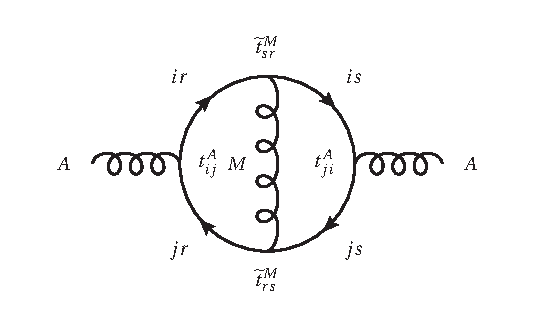
\includegraphics{abschnitte/n-schleifen/fig/QCDxdQCD1.eps}
 \caption*{(a)}
\end{minipage}
\begin{minipage}[t]{0.5\textwidth}
 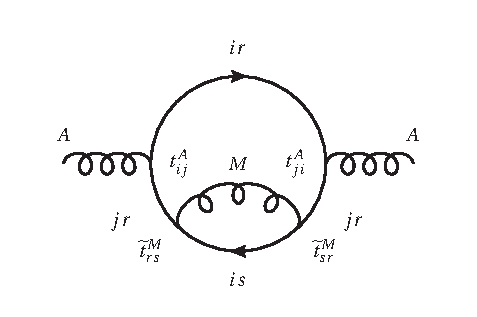
\includegraphics{abschnitte/n-schleifen/fig/QCDxdQCD2var.eps}
 \caption*{(b)}
 \end{minipage}
 \caption{2-Schleifen-Korrekturen $\propto (t^A_{ij})^2(\widetilde{t}^M_{rs})^2$ zum Gluonpropagator.}\label{fig:n-schleifen:QCDxdQCD2}
\end{figure}